\chapter{Test}
For at verificere systemets funktionaliteter for både hardware og software blev der udført modultests, integrationstests samt en endelig accepttest. I følgende afsnit vil fremgangsmåden for hver type test blive beskrevet, samt opsummerede resultater af udførte tests. 

\section{Modultest}
Ved modultests blev én funktionalitet testet isoleret, dvs. ved så lidt påvirkning fra resten af systemet som muligt. Modultests blev udført før integrationstests, for at sikre individuel funktionalitet før sammensætning af alle komponenter. Modultests blev udført både for software-komponenter og hardware-komponenter.

\subsection{Software}
Til modultest af software er der gjort brug af white-box testing. Dette er gjort, da softwaren ligger tæt op ad hardwaren til kommunikationsbusserne, hvilket kræver teknisk viden om den interne struktur for både hardware og software.

\subsubsection{Wii-Nunchuck}
Dataoverførsel fra Wii-Nunchuck sker ved at PSoC0 først sender et \textit{handshake}, hvilket er en enkelt byte med værdien 0x00. Herefter kan PSoC0 aflæse Wii-Nunchuck tilstanden ved kontinuert at sende en byte med værdien \textit{??}, efterfulgt af den egentlig aflæsning. Det er altså disse to dele der skal testes på.

For flere tekniske detaljer, samt billeder af målingerne, refereres til \textbf{DOKUMENTATION \#ref}

Tabel \ref{table:modulTestNunchuckHandShake} og \ref{table:modulTestNunchuckReading} præsenterer modultest resultaterne for Wii-Nunchuck.

\begin{table}[H]
	\centering
	\begin{tabular}{ll}
		\hline
		Forventet Resultat & \begin{tabular}[c]{@{}l@{}}På I2C Bussen måles et \textit{ACKNOWLEDGE} fra Wii-Nunchuck \\ slaven når den får tilsendt et handshake fra PSoC0. Det skal \\ desuden kunne ses at en byte med værdien 0x00 modtages \\ af Wii-Nunchuck. \end{tabular} \\
		\rowcolor[HTML]{CBCEFB} 
		Egentlig Resultat  & \begin{tabular}[c]{@{}l@{}}Et \textit{ACKNOWLEDGE} blev målt som forventet, \\ og handshake byten med værdi 0x00 blev modtaget korrekt. \end{tabular}                                       \\ \hline
	\end{tabular}
	\caption{Modultest af Wii-Nunchuck Handshake}
	\label{table:modulTestNunchuckHandShake}
\end{table}

\begin{table}[H]
	\centering
	\begin{tabular}{ll}
		\hline
		Forventet Resultat & \begin{tabular}[c]{@{}l@{}}På I2C bussen måles en aflæsning af bytes fra Wii-Nunchuck\\ slaven.\end{tabular}                \\
		\rowcolor[HTML]{CBCEFB} 
		Egentlig Resultat  & \begin{tabular}[c]{@{}l@{}}På målingen af I2C bussen ses det at bytes bliver aflæst fra\\ Wii-Nunchuck slaven.\end{tabular} \\ \hline
	\end{tabular}
	\caption{Modultest af Wii-Nunchuck Data Aflæsning}
	\label{table:modulTestNunchuckReading}
\end{table}

Det kan på tabel \ref{table:modulTestNunchuckHandShake} og \ref{table:modulTestNunchuckReading} ses at de egentlige resultaterne stemte overens med de forventede.

\subsubsection{I2C Kommunikationsprotokol}
I2C Kommunikationsprotokollen beskrevet i afsnit \ref{afsnit:I2CProtokol} blev modultestet ved to tests. Den første test er til for at verificere at kommandotyper bliver overført på I2C bussen i korrekt format. Den anden test er til for at verificere at modtaget I2C data fortolkes korrekt af software på PSoC0.

\begin{table}[H]
	\centering
	\begin{tabular}{ll}
		\hline
		Forventet Resultat & \begin{tabular}[c]{@{}l@{}}På I2C Bussen måles kommandotypen NunchuckData \\i korrekt format.\end{tabular} \\
		\rowcolor[HTML]{CBCEFB} 
		Egentlig Resultat  & \begin{tabular}[c]{@{}l@{}}Målingen af I2C bussen viste kommandotypen \\ NunchuckData i korrekt format.  \end{tabular}                                       \\ \hline
	\end{tabular}
	\caption{Modultest af kommandotype på I2C Bussen}
	\label{table:modulTestCommandFormat}
\end{table}

\begin{table}[H]
	\centering
	\begin{tabular}{ll}
		\hline
		Forventet Resultat & \begin{tabular}[c]{@{}l@{}} \end{tabular} \\
		\rowcolor[HTML]{CBCEFB} 
		Egentlig Resultat  & \begin{tabular}[c]{@{}l@{}}  \end{tabular}                                       \\ \hline
	\end{tabular}
	\caption{Modultest af kommandofortolkningssoftware}
	\label{table:modulTestI2CData}
\end{table}

\subsubsection{SPI Kommunikationsprotokol}

\subsubsection{Rotationsdetektor}
\begin{table}[H]
	\centering
	\begin{tabular}{|l|c|c|}
		\hline
		\textbf{Indgangssignal} & \textbf{Forventet PWM} & \textbf{Målt PWM} \\ \hline
		0V                      & Ja                     & Ja                \\ \hline
		1400mV                  & Ja                     & Ja                \\ \hline
		1500mV                  & Ja                     & Ja                \\ \hline
		1600mV                  & Nej                    & Ja                \\ \hline
		2,2V                    & Nej                    & Ja                \\ \hline
		2,3V                    & Nej                    & Nej               \\ \hline
		5V                      & Nej                    & Nej               \\ \hline
	\end{tabular}
	\caption{Modultest af ADC}
	\label{my-label}
\end{table}

\subsection{Hardware}

\subsubsection{Rotationsdetektor}
Der er udført en række modultests af rotationsdetektoren. Først er der en beskrivelse af testen, der skulle teste de forskellige dele i rotationsdetektorkredsløbet, både mens fotodioden modtager et lyssignal fra LED'en, og når den ikke gør. Herefter følger en beskrivelse af modultesten af det båndpasfilter, der indgår i rotationsdetektoren og til sidst er der en beskrivelse af modultesten af motorens PWM-signal. 

På figur \ref{fig:målepunkter} ses, hvor der er målt for at teste rotationsdetektoren. 

\begin{figure}[H]
	\centering
	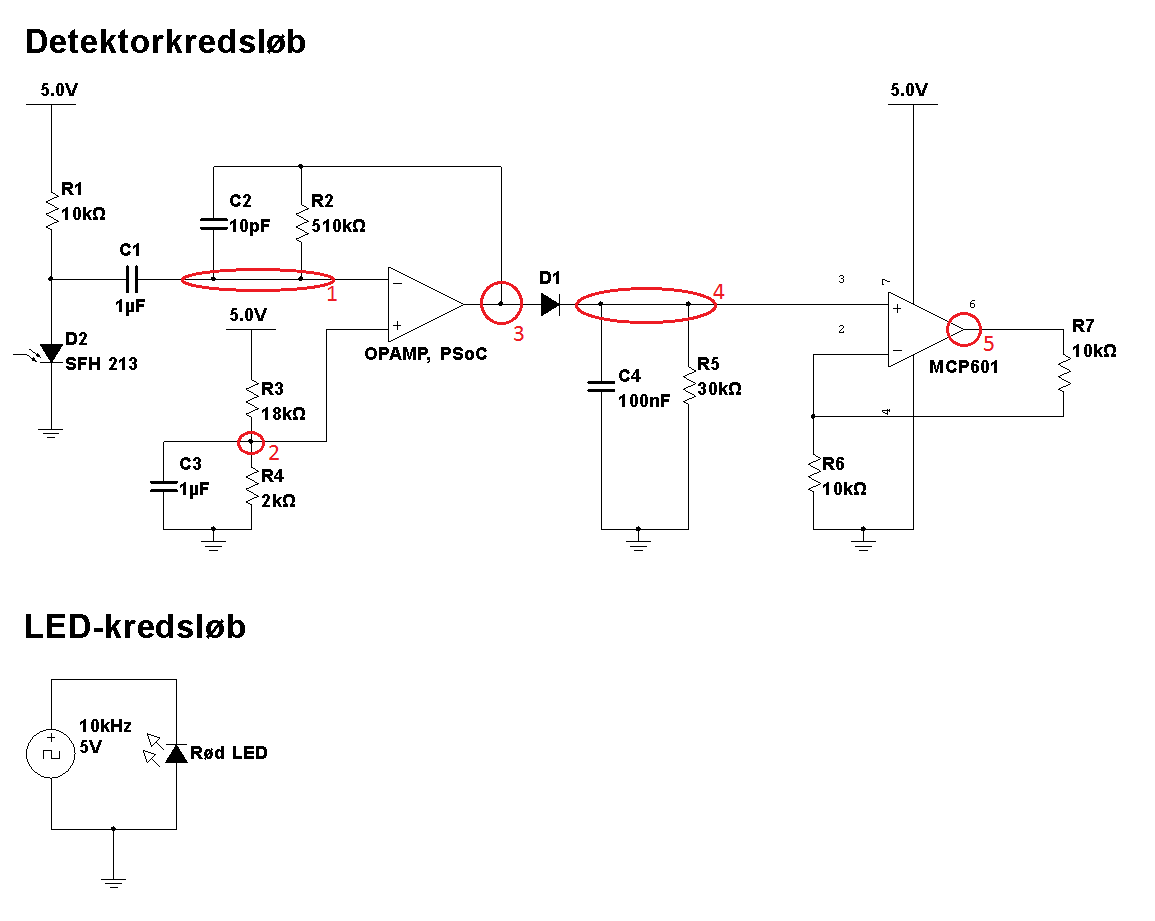
\includegraphics[width=\textwidth]{Test/images/rotationsdetektor_maalepunkter}
	\caption{Målepunkter på rotationsdetektor}
	\label{fig:målepunkter}
\end{figure}

I tabel \ref{dioderIkkeSe} ses resultaterne fra modultesten af rotationsdetektoren, når fotodioden ikke får noget lyssignal. Det ses, at det virtuelle nul fra spændingsdeleren ligger på 0,4V, og at forstærkeren fordobler signalet, hvilket var meningen. 

\begin{table}[H]
	\centering
	\begin{tabular}{|l|l|c|c|}
		\hline
		\textbf{Knudepunkt}		& \textbf{Målested}       & \textbf{Forventet resultat} & \textbf{Målt resultat} \\ \hline
		1						& Virtuelt 0              & 0,5V                        & 0,4V                   \\ \hline
		2						& Spændingsdeler          & 0,5V                        & 0,45V                  \\ \hline
		3						& Udgang på OpAmp på PSoC & 0,5V                        & 0,4V                   \\ \hline
		4 						& Envelope detector       & 0,5V                        & 0,4V                   \\ \hline
		5 						& Udgang på forstærker    & 1V                          & 0,85V                  \\ \hline
	\end{tabular}
	\caption{Modultest af rotationsdetektor, når fotodioden ikke modtager lyssignal fra LED}
	\label{dioderIkkeSe}
\end{table}

I tabel \ref{dioderSe} ses resultaterne fra modultesten af rotationsdetektoren, når fotodioden får lyssignal fra LED'en. Her ses det, at der igen er 0,4V, der hvor det var meningen, der skulle være 0,5V, så det er fint. Det ses også, at der er et PWM-signal på udgangen af PSoC'ens operationsforstærker og forstærkeren forstærker signalet, som ønsket. 

\begin{table}[H]
	\centering
	\begin{tabular}{|l|c|c|}
		\hline
		\textbf{Sted}           & \textbf{Forventet resultat} & \textbf{Målt resultat} \\ \hline
		Virtuelt 0              & 0,5V                        & 0,4V                   \\ \hline
		Spændingsdeler          & 0,5V                        & 0,45V                  \\ \hline
		Udgang på OpAmp på PSoC & PWM, 0-5V                   & PWM, 0-4V              \\ \hline
		Envelope detector       & \multicolumn{1}{l|}{}       & 3,7V                   \\ \hline
		Udgang på forstærker    & \multicolumn{1}{l|}{}       & 4,7V                   \\ \hline
	\end{tabular}
	\caption{Modultest af rotationsdetektor, når fotodioden modtager lyssignal fra LED}
	\label{dioderSe}
\end{table}

I tabel \ref{forstaerkerudgang} ses resultaterne fra modultesten af båndpasfilteret. 

\begin{table}[H]
	\centering
	\begin{tabular}{|l|c|c|}
		\hline
		\textbf{PWM-værdi} & \textbf{Forventet værdi} & \textbf{Målt værdi} \\ \hline
		40kHz              & \multicolumn{1}{l|}{}    & 3V                  \\ \hline
		29kHz              & \multicolumn{1}{l|}{}    & 3,9V                \\ \hline
		10kHz              & \multicolumn{1}{l|}{}    & 4,7V                \\ \hline
		10Hz               & \multicolumn{1}{l|}{}    & -                   \\ \hline
		5V (lyser LED?)    & Ja                       & Ja                  \\ \hline
	\end{tabular}
	\caption{Modultest af forstærkerudgangen}
	\label{table:forstaerkerudgang}
\end{table}

Afskæringsfrekvenserne for båndpasfilteret ligger på 15,9Hz og 31,2kHz, så hvis båndpasfilteret skulle være helt optimalt skulle alt, der ligger udenfor disse frekvenser dæmpes fuldstændig. Det ses dog i tabel \ref{forstaerkerudgang}, at det ikke helt er tilfældet. Ved 40kHz er signalet dæmpet til 3V, og ved 10kHz lader filteret alt gå igennem. Ved 10 Hz ses det, at signalet dæmpes, men der forekommer også mange spikes, som forstyrrer signalet. Derfor er der ikke indsat et tal i tabellen. 

\section{Integrationstest}

\section{Accepttest}